\documentclass[]{beamer}
% Class options include: notes, notesonly, handout, trans,
%                        hidesubsections, shadesubsections,
%                        inrow, blue, red, grey, brown

% Theme for beamer presentation.
\usepackage{beamerthemesplit} 
% Other themes include: beamerthemebars, beamerthemelined, 
%                       beamerthemetree, beamerthemetreebars  
\usepackage{amsmath}
\usepackage{mathtools}
\usepackage{amsfonts}
\usepackage{amssymb}
\usepackage{physics}
\usepackage{mathrsfs}
\title{Interaction-free measurements of different absorbers}    % Enter your title between curly braces
\author{Gerardo Suarez}                 % Enter your name between curly braces
\institute{Physics Department,\\ CINVESTAV}      % Enter your institute name between curly braces
\date{\today}                    % Enter the date or \today between curly braces

\begin{document}

% Creates title page of slide show using above information
\begin{frame}
  \titlepage
\end{frame}
\note{Talk for 30 minutes} % Add notes to yourself that will be displayed when
                           % typeset with the notes or notesonly class options

\section[Outline]{}

% Creates table of contents slide incorporating
% all \section and \subsection commands
\begin{frame}
  \tableofcontents
\end{frame}


\section{SPDC}

\begin{frame}
  \frametitle{SPDC in a nutshell}   % Insert frame title between curly braces

  \begin{itemize}
  \item Geometry of Type I SPDC
  \item Photon pair Production
  \item Spatial correlations in SPDC
  \end{itemize}
\end{frame}

\begin{frame}
\frametitle{A frame}
  \begin{columns}[T]
    \begin{column}{.5\textwidth}
     \begin{block}{Geometry of SPDC Type I}
     In SPDC type I, both photons travel on the same light-cone, both idler photons and signal photons have the same polarization which is orthogonal to the polarization of the pump photon
% Your text here
    \end{block}
    \end{column}
    \begin{column}{.5\textwidth}
    \begin{block}{}
% Your image included here
    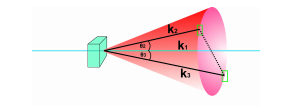
\includegraphics[width=\textwidth]{images/spdc_I.png}
    \end{block}
    \end{column}
  \end{columns}
\end{frame}

  \begin{frame}
    \frametitle{Photon Pair Production}
We will start our description of the SPDC process starting from the quantized electric field which can be written as:

\begin{align}
\textbf{E}(\textbf{r},t)=\textbf{E}^{(+)} (\textbf{r},t) + \textbf{E}^{(-)} (\textbf{r},t),\\
\textbf{E}^{(+)} (\textbf{r},t)=\frac{1}{\sqrt{V}} \sum_{\textbf{k},\nu} i(2 \pi \hbar w)^{\frac{1}{2}} \hat{a}_{\textbf{k},\nu} \hat{e}_{\textbf{k},\nu} e^{i(\textbf{k.r}-wt)}=[\textbf{E}^{(-)} (\textbf{r},t)]^{\star}
\end{align}
  \end{frame}

  \begin{frame}
    \frametitle{Photon Pair Production}
Now the hamiltonian of an electromagnetic field can be written as:

\begin{equation}
H=\frac{1}{2}\int_{V} d^{3}r (\textbf{D.E}+\textbf{H.B})
\end{equation}

where $\textbf{D}$ and $\textbf{H}$ are given by the constitutive equations:

\begin{align}
\textbf{D}= \epsilon_{0} \textbf{E}+\textbf{P},\\
\textbf{H}=\frac{\textbf{B}}{\mu_{0}}-\textbf{M}
\end{align}

Our system doesn't have magnetic field $\textbf{B}$ and we will neglect $\textbf{M}$ because we will assume that the laser beam is not strong enough to magnetize the crystal, so the hamiltonian becomes:

\begin{equation}
H=\frac{1}{2}\int_{V} d^{3}r \epsilon_{0}(\textbf{E.E}+\textbf{E.P})=H_{0}+H_{I}
\end{equation}



  \end{frame}

\begin{frame}
\frametitle{Photon Pair Production}
The term $H_{I}$ is the one that has to do with the interaction of the laser pump and the crystal so  it is the one we will be studying, we will consider the polarization to be nonlinear, however we will consider that the linear term is negligible and the main contributor to the process is the second term in the nonlinear expansion so(the expression for this second order polarization can be found in \cite{boyd}):


\begin{align}
H_{I}=\frac{\epsilon_{0}}{2} \int_{V} d^{3}r \textbf{E}.\textbf{P}^{(2)},\\
P_{i}^{(2)}=\int_{0}^{\infty}dt_{1}\int_{0}^{\infty}dt_{2} \chi_{ijk}^{(2')}(t-t_{1},t-t_{2}) E_{j}(\textbf{r},t_{1}) E_{k}(\textbf{r},t_{2})
\end{align}
\end{frame}

\begin{frame}
\frametitle{Photon Pair Production}
By substituting (12) in (11) and separating the fields in the creation and annihilation fields this can be written as:

\begin{align*}
& H_{I}=\frac{\epsilon_{0}}{2} \int_{V}\int_{0}^{\infty}dt_{1}\int_{0}^{\infty}dt_{2} \chi_{ijk}^{(2')}(E_{i}^{(+)}E_{j}^{(+)}E_{k}^{(+)}+E_{i}^{(-)}E_{j}^{(+)}E_{k}^{(+)}\\
& +E_{i}^{(-)}E_{j}^{(-)}E_{k}^{(+)}+E_{i}^{(+)}E_{j}^{(-)}E_{k}^{(+)}+E_{i}^{(+)}E_{j}^{(+)}E_{k}^{(-)}+\\
& E_{i}^{(-)}E_{j}^{(+)}E_{k}^{(-)}+E_{i}^{(-)}E_{j}^{(-)}E_{k}^{(-)}+E_{i}^{(+)}E_{j}^{(-)}E_{k}^{(-)}) 
\end{align*}

SPDC as we mentioned before is the annihilation of one photon and the creation of two, the only term compatible with this is $E_{i}^{(+)}E_{j}^{(-)}E_{k}^{(-)}$, and it's conjugate which means the reverse process, the other terms would not conserve energy in the case of SPDC so we eliminate them:

\begin{equation}
H_{I}=\int_{V} d^{3}r \chi_{ijk}^{(2)} (E_{i}^{(+)}E_{j}^{(-)}E_{k}^{(-)}+C.C.)
\end{equation}

\end{frame}

\begin{frame}
\frametitle{Photon Pair production}


Doing some algebra , and taking the first order in a Dyson series:

\begin{align*}
U_{1}\ket{\psi(t_{0})}=\frac{-i\chi}{\hbar} (2 \pi)^{4} \int d^{3}k_{s}\int d^{3}k_{i} \alpha_{p}(\mathbf{k_{s}}+\mathbf{k_{i}},w_{p})\\
\delta(w_{s}+w_{i}-w_{p})\ket{\alpha_{p},1_{s},1_{i}}
\end{align*}

If we define $\xi=\frac{-i\chi(2 \pi)^{4}}{\hbar} \int d^{3}k_{i} \int d^{3}k_{s}\delta(w_{s}+w_{i}-w_{p}) \delta(\mathbf{k_{p}}-\mathbf{k_{s}}-\mathbf{k_{i}})$ we can then rewrite in terms of operators as:

\begin{equation}
U_{1}\ket{\alpha_{p},0_{s},0_{i}}=\xi \hat{a_{p}}\hat{a_{s}^{\dagger}}\hat{a_{i}^{\dagger}}\ket{\alpha_{p},0_{s},0_{i}}
\end{equation}

\end{frame}

\begin{frame}
\frametitle{Spatial Correlations}

It can be shown that all information spatial correlations are contained in the following function:
\begin{equation}
\Phi_{s}(\mathbf{q_{i}},\mathbf{q_{s}})=N \int d^{2}q_{i} \int d^{2}q_{s} \Phi_{q}(\mathbf{q_{i}},\mathbf{q_{s}}) e^{-i \mathbf{q_{s}}.\mathbf{r_{s}}} e^{-i \mathbf{q_{i}}.\mathbf{r_{i}}}
\end{equation}

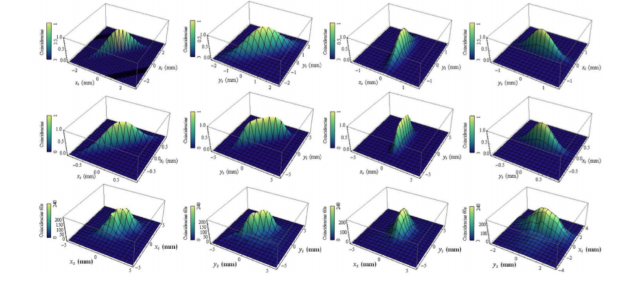
\includegraphics[width=\textwidth]{images/correlations.png}

\end{frame}

\begin{frame}
\frametitle{The Mach-Zehnder interferometer}
\includegraphics[width=\textwidth]{images/machzenhder.png}
\end{frame}
\begin{frame}
\frametitle{Classical Mach-Zehnder Interferometer}

We can calculate intensities with the following expressions:

\begin{align*}
I_{D1}=\abs{E_{1}}^2 (\rho^4 +\tau^4)(1+\frac{2 (\rho \tau)^2}{\rho^4+\tau^4}\cos(k\delta l)).\\
I_{D2}=\abs{E_{1}}^2 (\rho^4 +\tau^4)(1-\frac{2 (\rho \tau)^2}{\rho^4+\tau^4}\cos(k\delta l)).
\end{align*}

A case of interest is when $\rho=\tau=\frac{1}{\sqrt{2}}$, then the intensities become:

\begin{align*}
I_{D1}=\abs{E_{1}}^2 \frac{1+\cos(k \delta l)}{2}. \\
I_{D2}=\abs{E_{1}}^2 \frac{1-\cos(k \delta l)}{2}. 
\end{align*}


\end{frame}
\begin{frame}
\frametitle{Classical Mach-Zehnder Interferometer}


 
 For perfect alignment  $\delta l=\lambda n$ where n=1,2,3,..., so $\cos(2 \pi n )=1$ and the detector $D_{1}$ receives the intensity of the initial beam and $D_{2}$ receives no light.
 
\begin{align}
&I_{D1}=\abs{E_{1}}^2.\\
&I_{D2}=0.
\end{align}

\end{frame}

\begin{frame}
\frametitle{Single Photon Mach-Zenhder}


To Study a general situation, we will consider two different BS in our interferometer: 

\begin{align*}
& \ket{1}\xrightarrow{\text{BS1}}\cos(\theta_{1})\ket{1}+i\sin(\theta_{1})\ket{2}\xrightarrow{\text{Mirrors}}i\cos(\theta_{2})\ket{2}-\sin(\theta_{1})\ket{1}\\
&\xrightarrow{\text{BS2}} -(\cos(\theta_{1})\sin(\theta_{2})+\cos(\theta_{2})\sin(\theta_{1}))\ket{1}+\\
& i(\cos(\theta_{1})\cos(\theta_{2})-\sin(\theta_{1})\sin(\theta_{2}))\ket{2} 
\end{align*}


To compare with the classical case where we did our calculations with two identical BS we make $\theta_{1}=\theta_{2}=\frac{\pi}{4}$ then the state at the output of the interferometer is 

\begin{equation}
\ket{\psi}=-\ket{1}+0\ket{2}
\end{equation}

The probability to detect in $D_{1}$ is 1 and in $D_{2}$ is 0 , perfectly compatible with the result obtained in the classical case 

\end{frame}

\begin{frame}
\frametitle{Elitzur-Vaidman Bomb Detector}
We will denote an absorbed photon using the $\ket{Abs}$ state.
  
\begin{align*}
\ket{1}\xrightarrow{\text{BS1}}\cos(\theta_{1})\ket{1}+i\sin(\theta_{1})\ket{2}\xrightarrow{\text{Bomb}}\cos(\theta_{1})\ket{1}+i\sin(\theta_{1})\ket{Abs}\xrightarrow{\text{Mirrors}} \\
 i\cos(\theta_{1})\ket{2}+i\sin(\theta_{1})\ket{Abs}\xrightarrow{\text{BS2}}i\cos(\theta_{1})\cos(\theta_{2})\ket{2}-\cos(\theta_{1})\sin(\theta_{2})\ket{1}+i\sin(\theta_{1})\ket{Abs} 
\end{align*}

The probabilities to be absorbed or detected at either $D_{1}$ or $D_{2}$ are given by:

\begin{align}
P_{D1}=\cos^2(\theta_{1}) \sin^2(\theta_{2}) .\\
P_{D2}=\cos^2(\theta_{1}) \cos^2(\theta_{2}).\\
P_{Abs}=\sin^2(\theta_{1}).\\
\end{align}

\end{frame}

\begin{frame}
\frametitle{Elitzur-Vaidman Bomb}
Let us again consider the case where $\theta_{1}=\theta_{2}=\frac{\pi}{4}$ then:
\begin{equation}
P_{D1}=\frac{1}{4},P_{D2}=\frac{1}{4},P_{Abs}=\frac{1}{2}.
\end{equation}

A single Detection in $D_{2}$ can tell us whether an object is there or not without interacting with it 
\end{frame}

\begin{frame}
\frametitle{Mach-Zenhder Imperfect absorber}
In order to obtain all results with less effort it is way more comfortable to work in matrix notation: 
\begin{equation}
BS_{2}*M_{2}*M_{1}*A*BS_{1}\ket{Initial}
\end{equation}

so probabilities are given by:

\begin{equation}
P_{final}=|\bra{Final}BS_{2}*M_{2}*M_{1}*A*BS_{1}\ket{Initial}|^{2}
\end{equation}
\end{frame}


\begin{frame}
\frametitle{Mach-Zenhder Imperfect absorber}
If we consider N interferometers then this simply becomes: 
\begin{equation}
(BS M_{2} M_{1} A)^{N-1}BS\ket{Initial}
\end{equation}

so probabilities are given by:

\begin{equation}
P_{final}=|\bra{Final}(BS M_{2} M_{1} A)^{N-1}BS \ket{Initial}|^{2}
\end{equation}
\end{frame}



\end{document}







